%
% welle.tex
%
% (c) 2019 Prof Dr Andreas Müller, Hochschule Rapperswil
%
\documentclass[tikz]{standalone}
\usepackage{amsmath}
\usepackage{times}
\usepackage{txfonts}
\usepackage{pgfplots}
\usepackage{csvsimple}
\usetikzlibrary{arrows,intersections,math}
\begin{document}
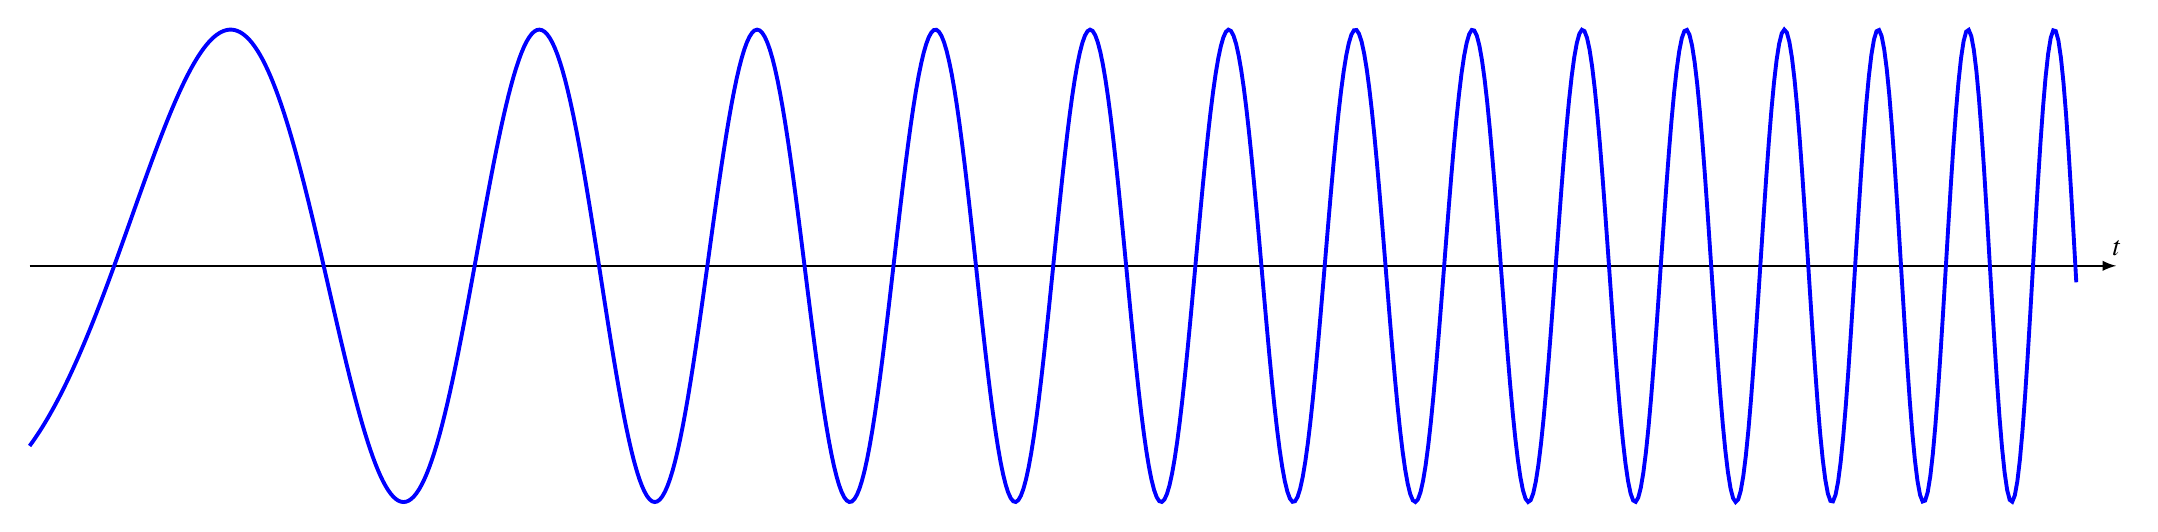
\begin{tikzpicture}[>=latex]

\def\pivalue{3.14159}

\draw[->,line width=0.7pt] (-13,0)--(13.5,0) coordinate[label={$t$}];

\draw[line width=1.4pt,color=blue] plot[domain=-13:13,samples=800]
	({\x},{3*sin(\x*(2+0.1*(\x+13))*(180/\pivalue))});

\end{tikzpicture}
\end{document}

